\documentclass[a4paper]{article}

\usepackage[czech]{babel} %https://github.com/michal-h21/biblatex-iso690
\usepackage[
   backend=biber      % if we want unicode 
  ,style=iso-numeric % or iso-numeric for numeric citation method          
  ,babel=other        % to support multiple languages in bibliography
  ,sortlocale=cs_CZ   % locale of main language, it is for sorting
  ,bibencoding=UTF8   % this is necessary only if bibliography file is in different encoding than main document
]{biblatex}

\usepackage[utf8]{inputenc}
\usepackage{fancyhdr}
\usepackage{amsmath}
\usepackage{amssymb}
\usepackage[left=2cm,right=2cm,top=2.5cm,bottom=2.5cm]{geometry}
\usepackage{graphicx}
\usepackage{pdfpages}
\usepackage{url}
\usepackage{multirow}

\usepackage{siunitx}
\sisetup{locale = DE}  %, separate-uncertainty = true    kdybych chtel +/-

\usepackage{float}
\newfloat{graph}{htbp}{grp}
\floatname{graph}{Graf}
\newfloat{tabulka}{htbp}{tbl}
\floatname{tabulka}{Tabulka}

\renewcommand{\thefootnote}{\roman{footnote}}

\pagestyle{fancy}
\lhead{Praktikum II - (6) Měření účiníku}
\rhead{Vladislav Wohlrath}
\author{Vladislav Wohlrath}

\bibliography{source}

\begin{document}

\begin{titlepage}
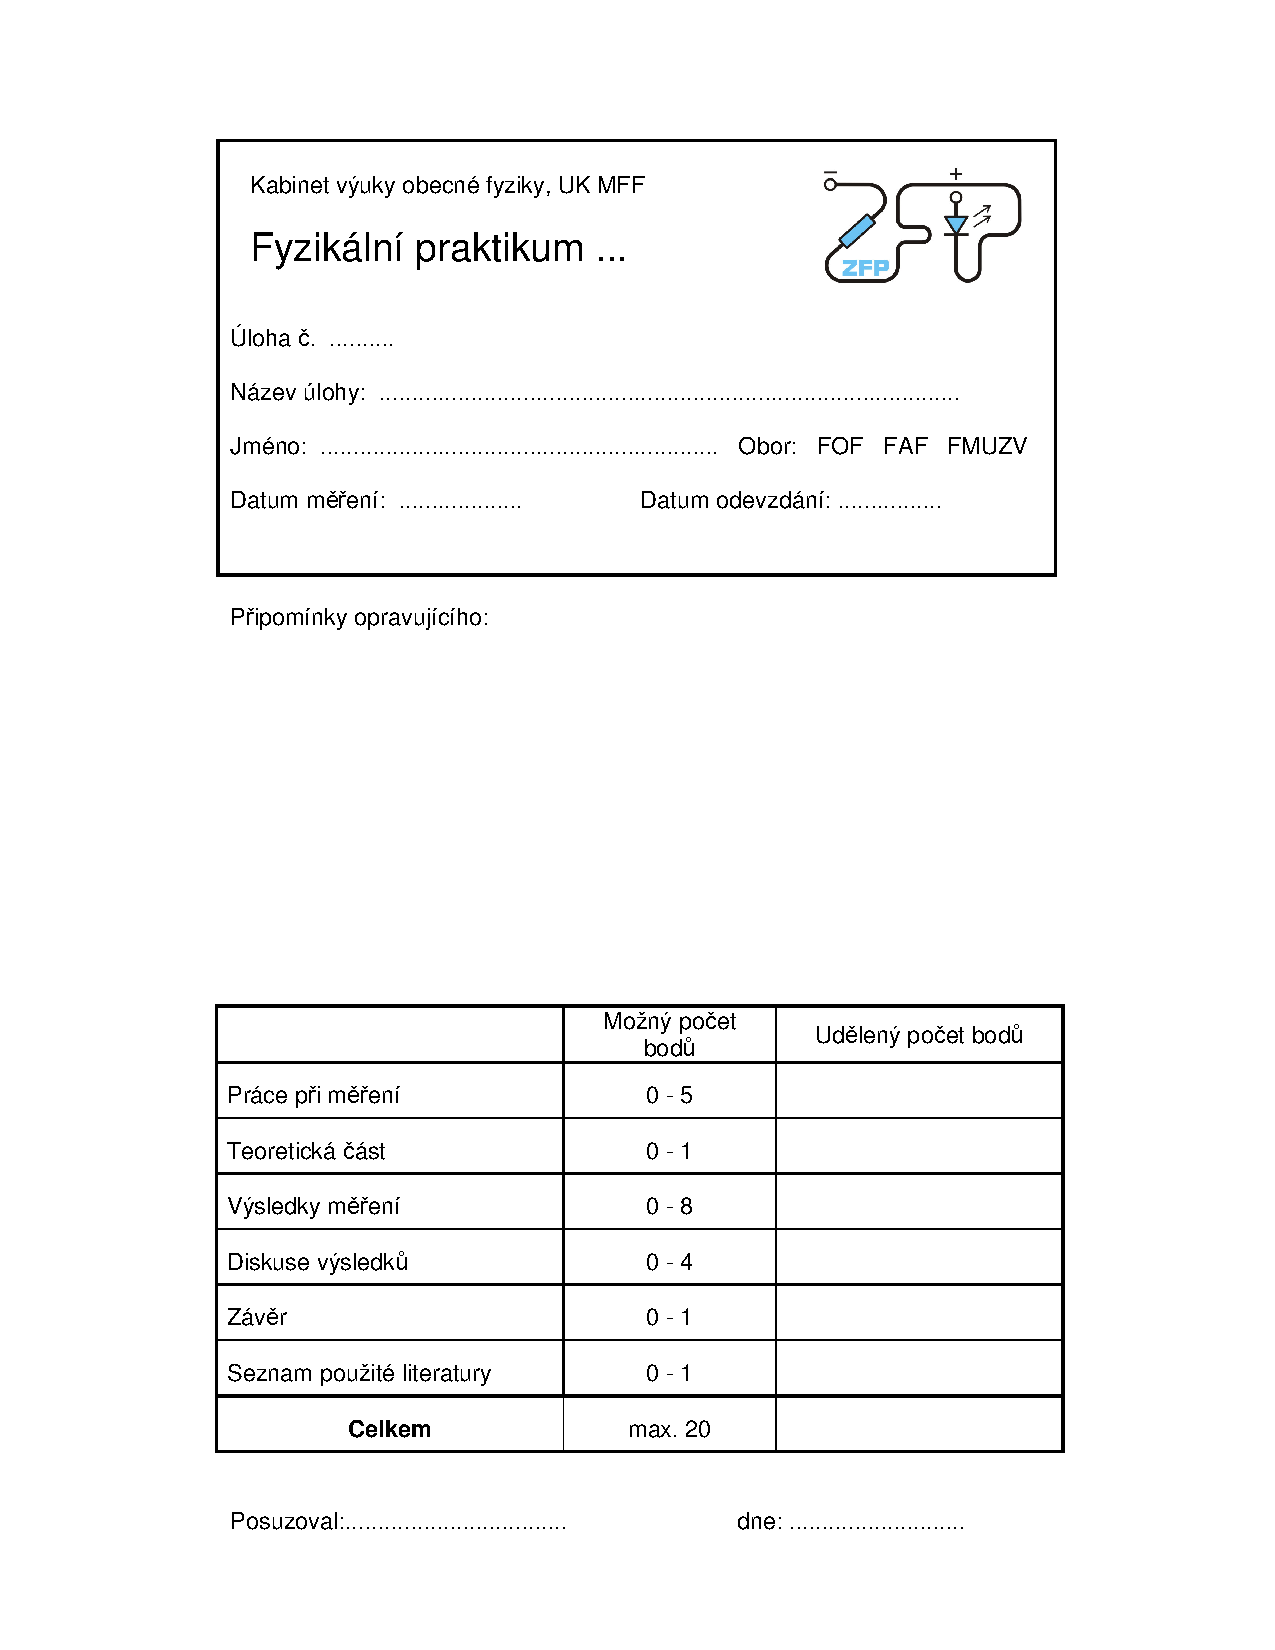
\includepdf[pages={1}]{./graficos/titlelist.pdf}
\end{titlepage}

\section*{Pracovní úkoly}
\begin{enumerate}
\item Změřte účiník:
\begin{enumerate}
\item rezistoru,
\item kondenzátoru ($C=\SI{10}{\micro\farad}$),
\item cívky.
\end{enumerate}
\item Spočtěte fázový posun proudu a napětí. Určete chybu měření. Diskutujte shodu výsledků s teoretickými hodnotami pro ideální prvky.
\item Pro cívku vypočtěte indukčnost a odpor v sériovém a paralelním náhradním zapojení.
\item Změřte účiník sériového a paralelního zapojení rezistoru a kondenzátoru pro kapacity v intervalu $C$ =  \mbox{1--\SI{10}{\micro\farad}} a spočtěte fázový posuv. Výsledky zpracujte graficky. Z naměřených hodnot stanovte odpor rezistoru a porovnejte ho s hodnotou přímo naměřenou digitálním multimetrem. Určete chyby měření a rozhodněte, které z obou zapojení je v daném případě vhodnější pro stanovení odporu.
\item Změřte závislost proudu a výkonu na velikosti kapacity zařazené do sériového RLC obvodu pro kapacity do \SI{10}{\micro\farad}. Výsledky zpracujte graficky, v závislosti na zařazené kapacitě vyneste účiník, fázový posuv napětí vůči proudu a výkon.
\item V průběhu měření seriového RC obvodu připojte na kondenzátor digitální osciloskop Tektronix a pozorujte změnu fáze napětí na kondenzátoru vzhledem k průběhu napětí zdroje v závislosti na velikosti nastavené kapacity v intervalu 1--\SI{10}{\micro\farad}. Popište kvalitativně pozorované jevy a vysvětlete je. Stručný popis ovládání a schema připojení osciloskopu je přiloženo u úlohy.


\end{enumerate}

%Teoretická část
\section*{Teoretická část}

%Výsledky měření
\section*{Výsledky měření}

%Diskuze výsledků
\section*{Diskuze}
Měření digitálním osciloskopem bylo v tomto případě přesnější než analogovým, protože na analogovém jsme měřili ve spodní části rozsahu.
U digitálního wattmetru bylo velkou chybou zatíženo měření proudu ze stejného důvodu.
Nicméně výsledky získané oběma přístroji se poměrně přesně shodují.


U rezistoru nám podle očekávání vyšel účiník 1.
U kondenzátoru vyšel téměř přesně 0, takže ho můžeme považovat za ideální a jeho vlastní vodivost zanedbat.
U cívky vyšel účiník \num{0.41}, takže má nezanedbatelný odpor.

Měření odporu pomocí účiníku RC obvodu bylo přesnější v paralelním zapojení, a to zejména kvůli již zmiňované nepřesnosti měření proudu. Vypočtené odpory se v rámci chyby přibližně shodují pro všechna měření a shodují se i s hodnotou naměřenou multimetrem.
Měření multimetrem považujeme v tomto případě za přesnější.

%Závěr
\section*{Závěr}
Změřili jsme účiník a fázový posuv rezistoru, kondenzátoru a cívky, viz tabulka \ref{t:jednicka}.

Zjistili jsme, že rezistor a kondenzátor lze pro naše účely považovat za ideální.
Cívka má účiník různý od jedné, takže ji nelze považovat za ideální. Vypočítali jsme indukčnost a odpor v sériovém a paralelním náhradním zapojení. V sériovém zapojení
\begin{equation*}
R_S=\SI{720(50)}{\ohm}  \qquad \qquad L_S=\SI{5.1(2)}{\henry}
\end{equation*}
a v paralelním
\begin{equation*}
R_P=\SI{4270(50)}{\ohm} \qquad \qquad L_P=\SI{6.1(2)}{\henry} \,.
\end{equation*}

Změřili jsme účiník sériového a paralelního RC obvodu, viz tabulka \ref{t:RC} a grafy \ref{g:RCucinik} a \ref{g:RCfaze}. Pomocí něj jsme určili odpor $R = \SI{990(5)}{\ohm}$. Odpor jsme změřili i digitálním multimetrem na \SI{982(2)}{\ohm}.

Změřili jsme závislost proudu a výkonu na velikosti kapacity zařazené do sériového RLC obvodu, viz přiložená tabulka a grafy \ref{g:RLCu}, \ref{g:RLCf} a \ref{g:RLCP}.


\printbibliography[title={Seznam použité literatury}]

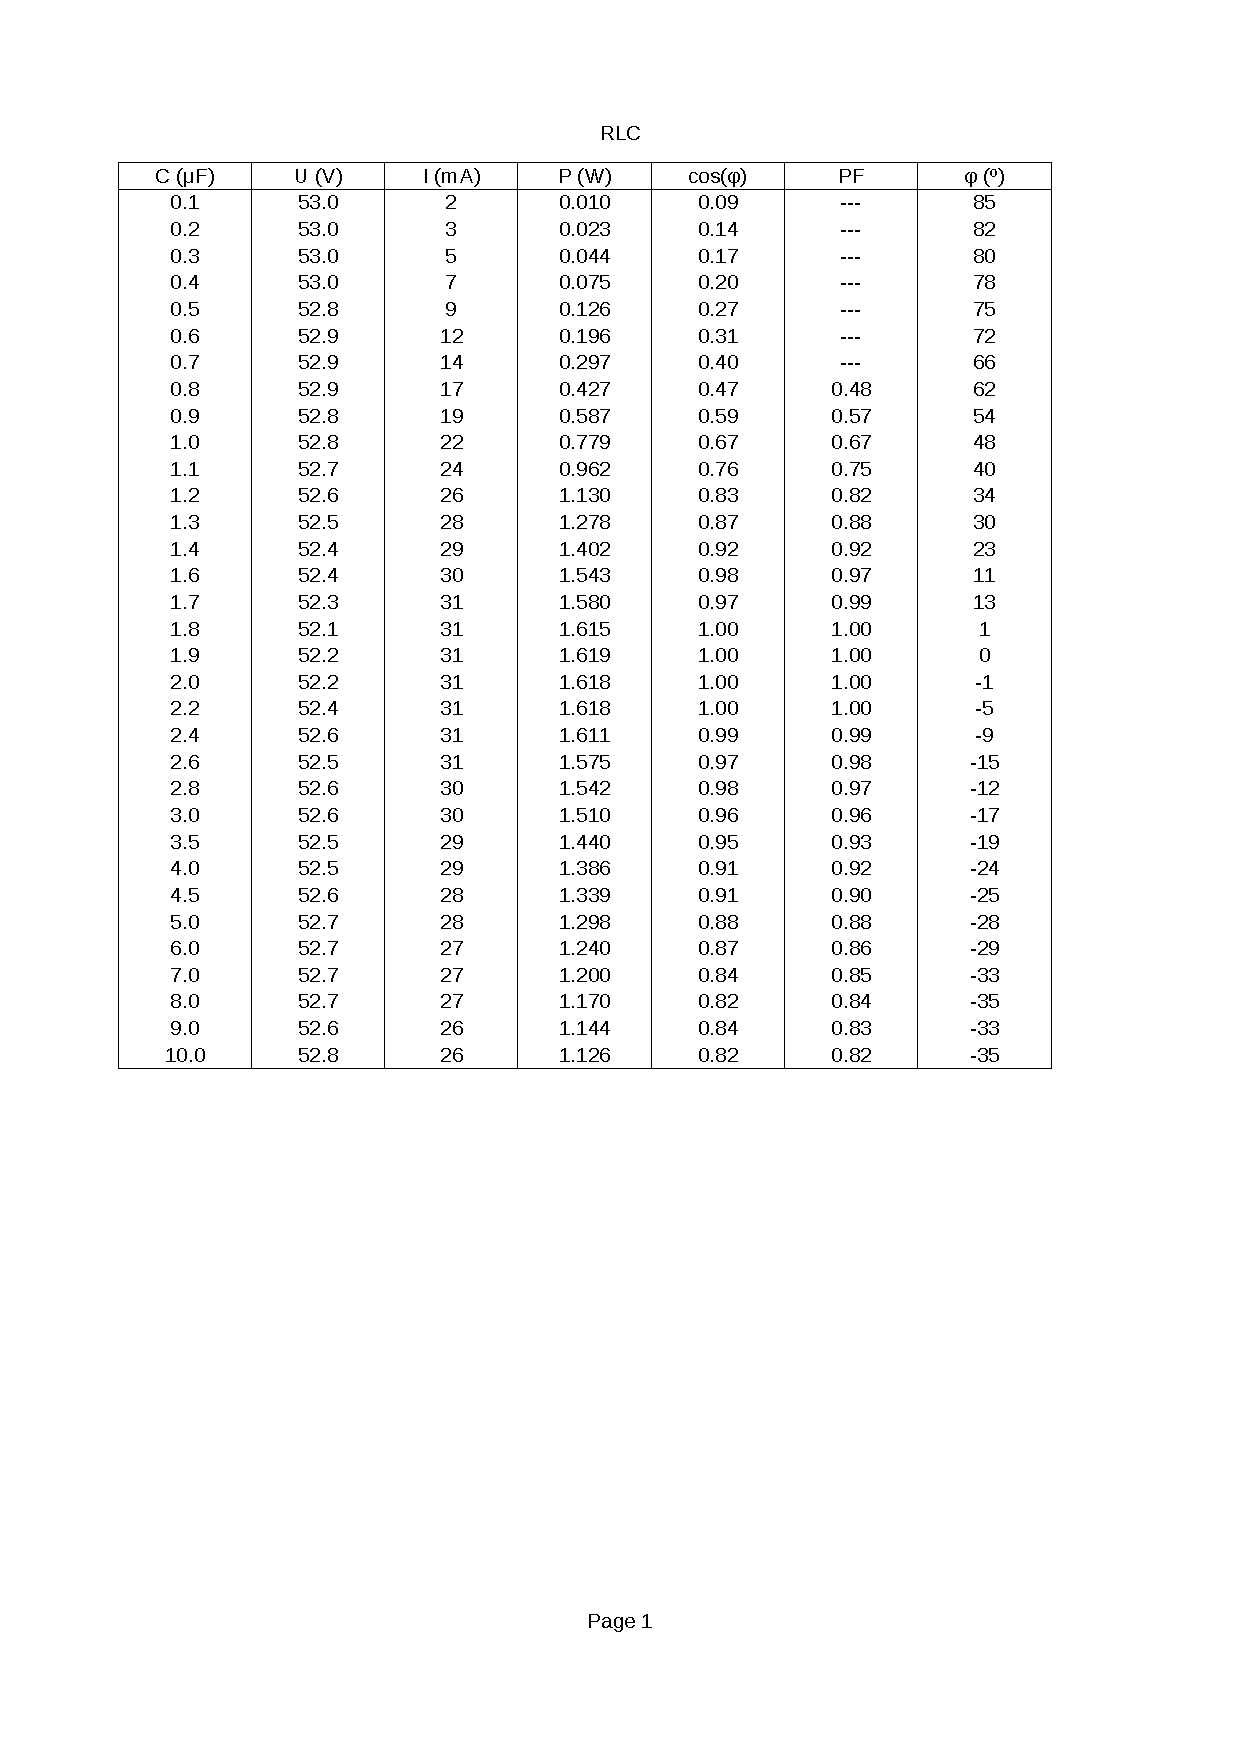
\includepdf[pages={1}]{./tabulka.pdf}

\end{document}